\section{Non-Preemptive Protocol}

\subsection{Definition}

This protocol is a simple protocol and named non preemptive because it avoid any interruption on running task $\tau_{j}$ that accessing a resource $ R_{k} $that guarded by , $ S_{k} $. To reduce total blocking time experienced by the task $\tau_{i}$ that have highest priority, this protocol just increase the priority of the task $\tau_{j}$ that currently accessing the resource $\tau_{j}$, so that the task will not be interrupted and can be done much faster.Without this protocol, the task that highest priority $\tau_{i}$ will interrupt the task $\tau_{j}$ that currently accessing the resource $ R_{k} $ even though the task cannot access the resource because it already guarded by $ S_{k} $. The scheduler then switch back to the task before to finish its process, this switch context process could cause longer blocking time experienced by the highest priority task. After the task$\tau_{j}$ finish accessing the resources, its priority will be back to its nominal priority $ P_{j} $.These situations can be compared through figure \ref{fig:An_example_of_priority_inversion} and \ref{fig:Example_of_NPP_preventing_priority_inversion} . So, the priority of the task $\tau_{i}$that currently accessing the resource is 

\begin{center}
$p_{i}(R_{k})=\underset{h}{\mathrm{max}} \{P_{h}\}  $

\end{center}

\begin{figure}[h]
    \centering
    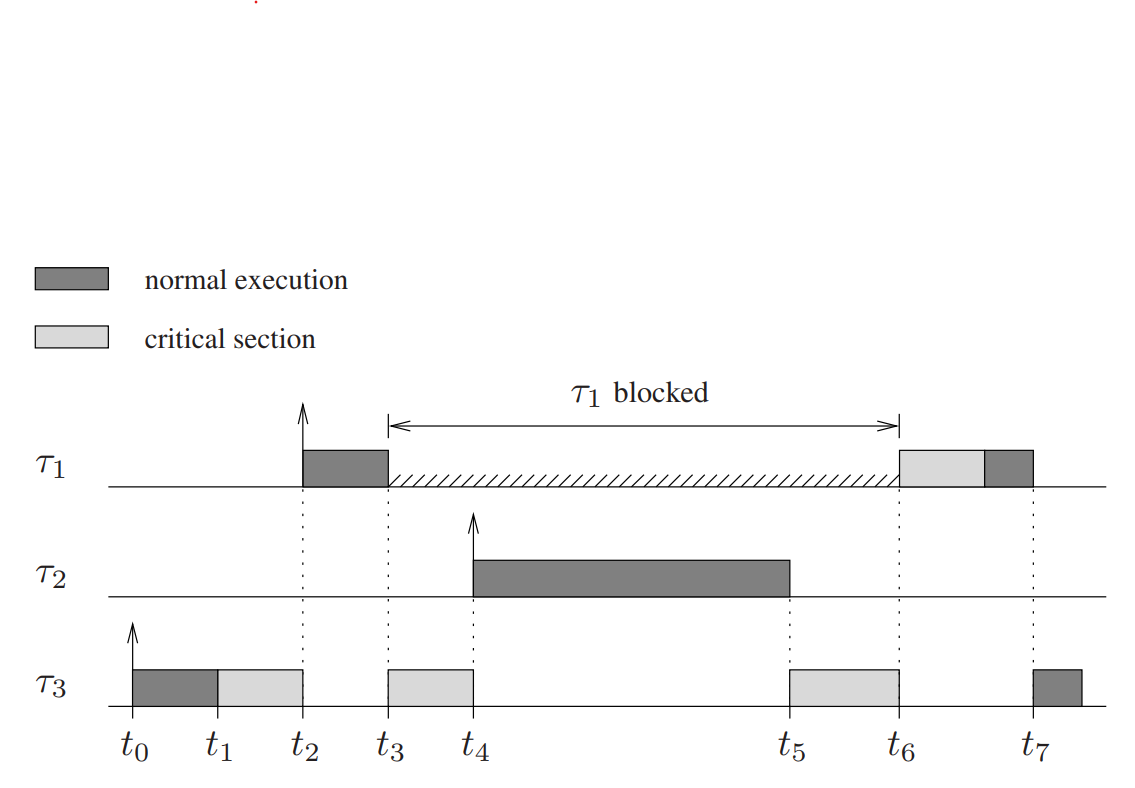
\includegraphics[width=0.5\textwidth]{An_example_of_priority_inversion}
    \caption{An example of priority inversion.. \cite{b5}}
    \label{fig:An_example_of_priority_inversion}
\end{figure}

\begin{figure}[h]
    \centering
    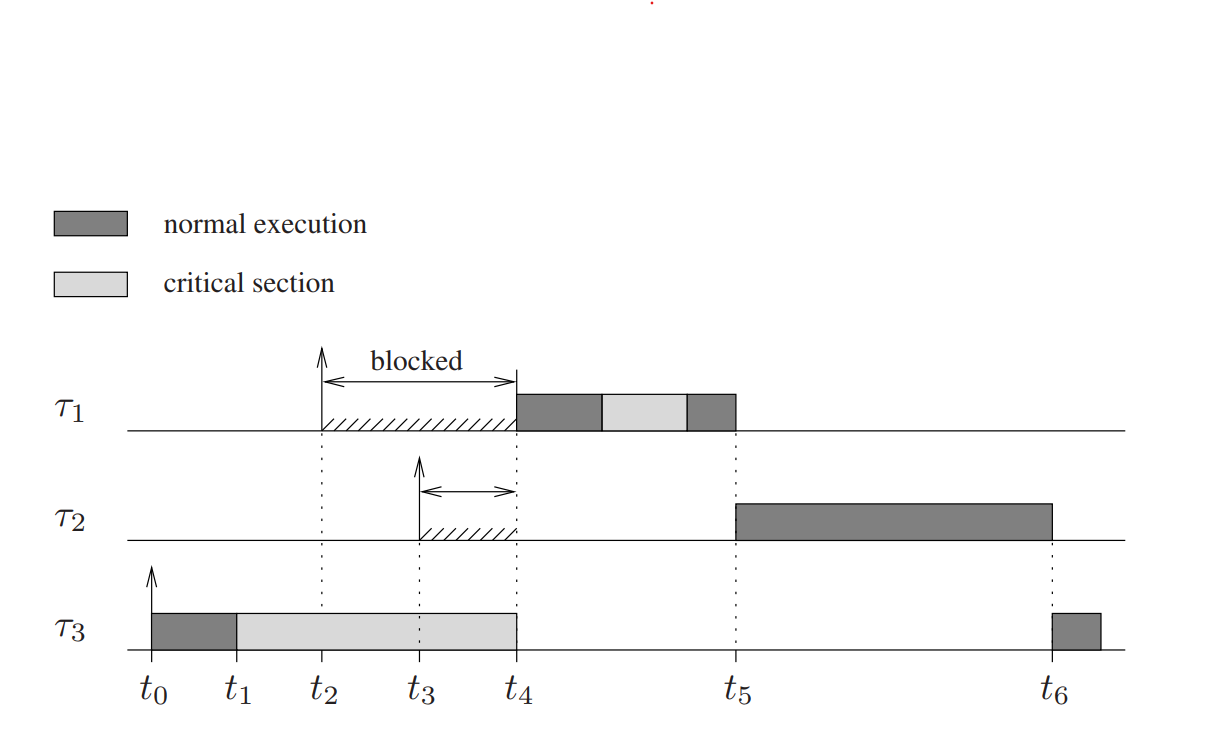
\includegraphics[width=0.5\textwidth]{Example_of_NPP_preventing_priority_inversion}
    \caption{Example of NPP preventing priority inversion. \cite{b5}}
    \label{fig:Example_of_NPP_preventing_priority_inversion}
\end{figure}


\subsection{Blocking time computation}

	The total of critical section of lower priority task $\tau_{j}$ blocking higher priority task $\tau_{i}$ is

\begin{center}
$ \gamma_{i}=\{Z_{j,k} | P_{j}<P_{i}, k=1,...,m \} $
\end{center}

Hence the total duration highest priority task is blocked is

\begin{center}

$B_{i}(R_{k})=\underset{j,k}{\mathrm{max}} \{ \delta_{j,k}-1 | Z_{j,k} \in \gamma_{i}\}  $
\end{center}

\subsection{Problem Arise}

As shown in figure \ref{fig:Example_in_which_NPP_causes_unnecessary_blocking_on_T1}, this protocol will block highest priority task $ \tau_{1} $ even though the task will not access the resource.This problem could be solved in the next protocol which is Highest Locker Priority (HLP) protocol.

\begin{figure}[h]
    \centering
    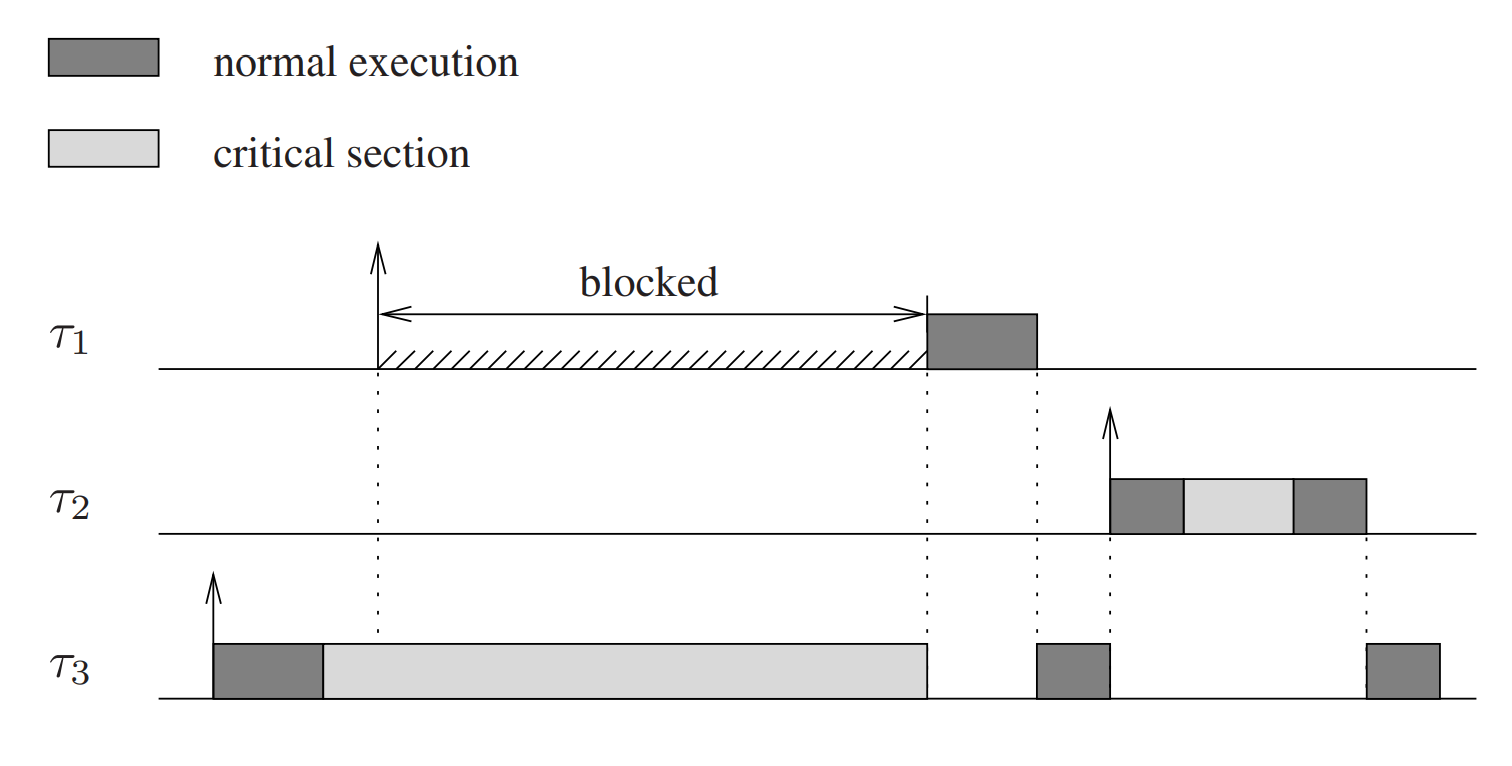
\includegraphics[width=0.5\textwidth]{Example_in_which_NPP_causes_unnecessary_blocking_on_T1}
    \caption{Example in which NPP causes unnecessary blocking on $ \tau_{1} $ \cite{b5}}
    \label{fig:Example_in_which_NPP_causes_unnecessary_blocking_on_T1}
\end{figure}



 
